\chapter{Results}

This chapter will summarize the results achieved with the \ac{PTINY} dialogue system.
We will describe the 2014 \ac{MTA} App Quest admission in the first part.
Then we will go through the subjective user satisfaction results collected from CrowdFlower.
And finally we will compare the subjective user satisfaction between the Google and Kaldi \ac{ASR}.

\section{App Quest 3.0}

At the beginning of February 2014, we participated in the contest App Quest 3.0\footnote{\url{http://2014mtaappquest.challengepost.com/}} by \acf{MTA}\footnote{\url{http://www.mta.info/}}.
The contest rules allowed registering teams and individuals around the globe and required to submit an application that utilizes at least one of the \ac{MTA} data sets or \acp{API} and includes the ability to update the data.

We registered in the Accessibility Innovation category because the primary features and functionality of \ac{PTINY} best addresses end user with visual impairment.
Our keyword database can be actualized any time from the server and we utilize \ac{MTA} data sets, therefore \ac{PTINY} is eligible to participate.

The application was, however, required to run on one of many mobile or desktop platforms.
The \ac{PTINY} is rather a phone service, therefore we decided to create a web page that enhances the accessibility even more.

A US number was provided by the department for the competition and three \acp{VM} were employed.
We submitted \ac{PTINY}\footnote{\url{http://challengepost.com/software/alex-information-about-public-transportation-in-new-york}} as an operational dialogue system, despite the fact that some features were not yet finished.

\subsubsection{\ac{PTINY} web page}

The web page\footnote{\url{http://alex-ptien.com/}} created for the competition contains the overview of \ac{PTINY}, examples of the features, terms of use and most importantly a ``try it now'' section shown in figure \ref{fig:mta}, in which a visitor has the opportunity to call \ac{PTINY} directly through the web page.

\begin{figure}[ht]
\centering
\includegraphics[width=0.9\linewidth]{../img/mta.eps}
\caption{Web page with the \textit{"Call us Now"} button for the 2014 \ac{MTA} App quest.}
\label{fig:mta}
\end{figure}

We utilized webrtc2sip gateway\footnote{\url{http://click2dial.org/u/index.html}} to create a \textit{Call us Now} button.
It allows any web browser supporting WebRTC protocol to call our \ac{SIP} account and to try out \ac{PTINY} without the need of calling a number.
This includes mobile devices, too.

One additional \ac{VM} was used for handling the button calls.

\subsubsection{\ac{PTINY} demonstration video}

Another requirement was to provide a video link along with the submission.
The video should clearly explains the features and functionality through a comprehensive demonstration.
With the help of my colleague's voice, we created a video demonstrating the features by an example call with detailed description. \footnote{\url{https://youtu.be/wtlFCJj8faE}}
We also elevated the fact, that it can be a great asset for the visually impaired.

\subsubsection{Competition results}

Unfortunately we were not among the winners and there was no ranking either, so we do not know how close to winning we were.
Even more disappointing was the fact that we collected virtually zero calls.
As the rules state, judges are not required to test the application and may choose to judge based solely on the text description or demonstration video.
Our hope was that \ac{PTINY} would attract at least the curiosity of some other competitors.

We know for certain that our solution scored poorly in one of the judging criteria which was utilizing \ac{MTA} \ac{API}.
We only utilize \ac{MTA} datasets.

However, the thing we cherish the most about our solution is that, while others were competing among each other within the same class of mobile applications, \ac{PTINY} brought a new point of view on providing information about public transportation, with which a human can simply chat.

\section{CrowdFlower -- subjective user satisfaction}

Every call job we launched on CrowdFlower had the same feedback form with questions listed in table \ref{table:cf}.
These questions measure the quality of every component of the dialogue system.
The first question about achieving objectives evaluates the whole dialogue system, especially \ac{DM}.
The second question about system phrasing measures the quality of \ac{NLG} , while the third one about the voice quality is concerned with \ac{TTS}.
And the last question asking about how the system understood the caller evaluates the \ac{ASR} and \ac{SLU} components.


\begin{table}[h]
\centering
\hspace*{-3pt}\makebox[\linewidth][c]{
	\begin{tabular}{ r | p{0.6\linewidth} }
	\textit{Have you found what you were looking for?} & Yes-No question \\
	\textit{The phrasing of the system's response was:} & range of 1 to 4 from Very poor to Very good \\
	\textit{The quality of the system's voice was:} & range of 1 to 4 from Very poor to Very good \\
	\textit{The system understood me:} & range of 1 to 4 from Very poorly to Very well \\
\end{tabular}
}
\caption[CrowdFlower feedback form questions]{CrowdFlower feedback form questions with choice ranges.}
\label{table:cf}
\end{table}

The results from each CrowdFlower job provided in a \ac{CSV} document were collected and joined for corresponding \ac{ASR}.
Even with the feedback form fields marked as mandatory, there were a few missing values in the results.
Thus we collected less feedback forms than calls.

In addition to the compulsory questions evaluating the job, there was an optional general comments field.
Comments gave a good overall image of the contributor satisfaction as they could express themselves freely and in few cases, they helped enhance the system.

\subsection{Google ASR}

It is important to note that the results from CrowdFlower call jobs that contributed to the Google \ac{ASR} evaluation were collected while some features of the system were not yet implemented.
However, the call job always encouraged callers to address only the features and functionalities working well.
Therefore the user satisfaction should not be influenced by the fact that the system changed over time.

% \begin{figure}[ht]
% \begin{tikzpicture}
% \begin{axis}[
%     every axis plot post/.style={/pgf/number format/fixed},
%     ybar,
%     x=4cm,
%     ymin=0,
%     ylabel = Number of votes,
%     %ymax=12,
%     legend columns=-1,
% 	legend style={at={(0.5,-0.2)},anchor=north},
%     xtick=data,
%     enlarge x limits=0.2,
%     bar width=15pt,
%     symbolic x coords={1, 2, 3, 4},
%     nodes near coords,
%     axis lines*=left,
%     xticklabels={System phrasing, Voice Quality, System understanding},
%     xtick={1,...,3},
%     ]

% \addplot[red!20!black,fill=red!80!white] coordinates {(1,24) (2,33) (3,37)};
% \addplot[orange!20!black,fill=orange!80!white] coordinates {(1,52) (2,57) (3,63)};
% \addplot[blue!20!black,fill=blue!80!white] coordinates {(1,127) (2,129) (3,120)};
% \addplot[green!20!black,fill=green!80!white] coordinates {(1,166) (2,150) (3,149)};
% \legend{Very poor, Poor, Good, Very good}
% \end{axis}
% \end{tikzpicture}
% \caption{Google subjective user satisfaction histograms for questions 2-4 from table \ref{table:cf}}
% \label{fig:google}
% \end{figure}

\begin{figure}[ht]
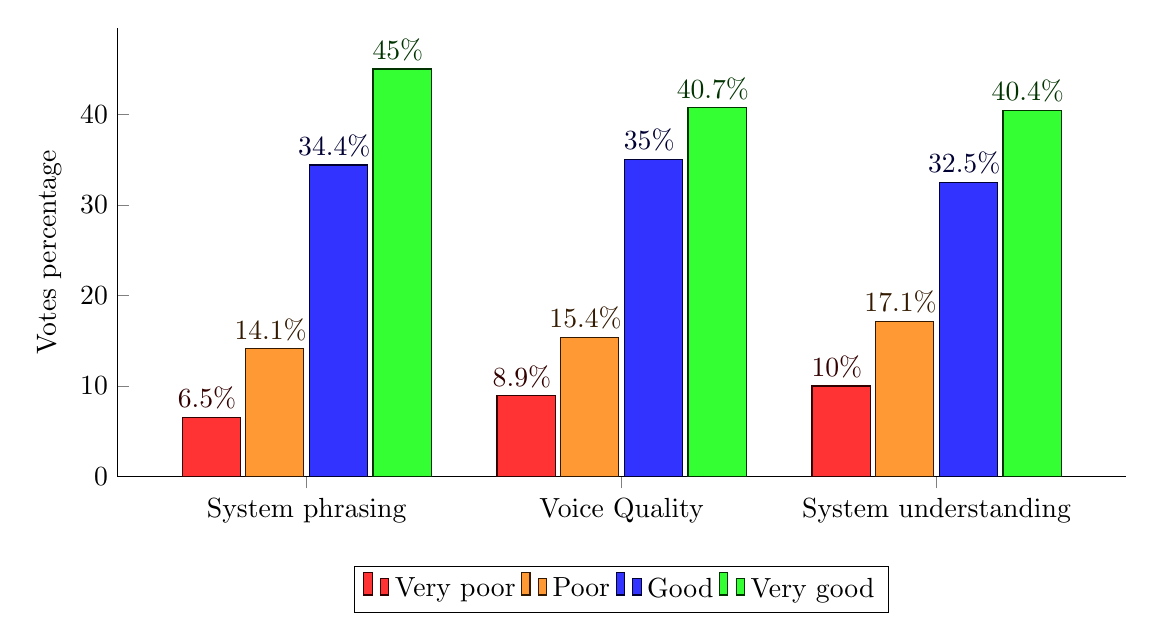
\begin{tikzpicture}
\begin{axis}[
    every axis plot post/.style={/pgf/number format/fixed},
    ybar,
    x=4cm,
    ymin=0,
    ylabel = Votes percentage,
    %ymax=12,
    legend columns=-1,
	legend style={at={(0.5,-0.2)},anchor=north},
    xtick=data,
    enlarge x limits=0.3,
    bar width=21pt,
    symbolic x coords={1, 2, 3, 4},
    nodes near coords={\pgfmathprintnumber\pgfplotspointmeta\%},
    nodes near coords align={
     shift={(-0.15em,0.7em)},
    },
    axis lines*=left,
    xticklabels={System phrasing, Voice Quality, System understanding},
    xtick={1,...,3},
    ]

\addplot[red!20!black,fill=red!80!white] coordinates {(1,6.5) (2,8.9) (3,10)};
\addplot[orange!20!black,fill=orange!80!white] coordinates {(1,14.1) (2,15.4) (3,17.1)};
\addplot[blue!20!black,fill=blue!80!white] coordinates {(1,34.4) (2,35) (3,32.5)};
\addplot[green!20!black,fill=green!80!white] coordinates {(1,45) (2,40.7) (3,40.4)};
\legend{Very poor, Poor, Good, Very good}
\end{axis}
\end{tikzpicture}
\caption{Google subjective user satisfaction histograms for questions 2-4 from table \ref{table:cf}}
\label{fig:google}
\end{figure}


We launched seven jobs with increasing number of ordered calls each time.
In the settings, we allowed contributors to participate only once per job to collect diverse data which caused the job to be rather unattractive, hence the collection quite slow.

Totally, we collected 369 valid feedback forms.
The figure \ref{fig:google} shows histograms of questions 2, 3 and 4.
It is clear that more than a half of callers were satisfied with the service.
The first yes-no overall question is shown in figure \ref{fig:us}.

In the general comment section, 101 contributors shared a mixture of positive and negative comments.

\begin{flushleft}
\textit{``Awful system - not working at all.''} \\
\textit{``Good service, no problems.''} \\
\textit{``It made me do it twice before it heard me.''} \\
\textit{``Excellent directions.''} \\
\end{flushleft}

\noindent This short list is a sample of repetitive comments in similar vein.

\subsection{Kaldi ASR}

The same setup of CrowdFlower call jobs was used when launching the same rate of tasks as in the case of Google \ac{ASR}.
We have collected five jobs with 280 valid feedback forms.
All of those five jobs had unique configuration urging callers to ask about different particular features and waypoints.
It was the same set of configuration as in the case of Google jobs, however two of those configurations were split into separate jobs due to development process.
This is why Google has more jobs and it only means that contributors could participate in jobs with those two configurations twice.

% \begin{figure}[ht]
% \begin{tikzpicture}
% \begin{axis}[
%     every axis plot post/.style={/pgf/number format/fixed},
%     ybar,
%     x=4cm,
%     ymin=0,
%     ylabel = Number of votes,
%     %ymax=12,
%     legend columns=-1,
% 	legend style={at={(0.5,-0.2)},anchor=north},
%     xtick=data,
%     enlarge x limits=0.2,
%     bar width=15pt,
%     symbolic x coords={1, 2, 3, 4},
%     nodes near coords,
%     axis lines*=left,
%     xticklabels={System phrasing, Voice Quality, System understanding},
%     xtick={1,...,3},
%     ]

% \addplot[red!20!black,fill=red!80!white] coordinates {(1,3) (2,8) (3,7)};
% \addplot[orange!20!black,fill=orange!80!white] coordinates {(1,21) (2,25) (3,31)};
% \addplot[blue!20!black,fill=blue!80!white] coordinates {(1,111) (2,98) (3,106)};
% \addplot[green!20!black,fill=green!80!white] coordinates {(1,134) (2,138) (3,125)};
% \legend{Very poor, Poor, Good, Very good}
% \end{axis}
% \end{tikzpicture}
% \caption{Kaldi subjective user satisfaction histograms for questions 2-4 from table \ref{table:cf}}
% \label{fig:kaldi}
% \end{figure}

\begin{figure}[ht]
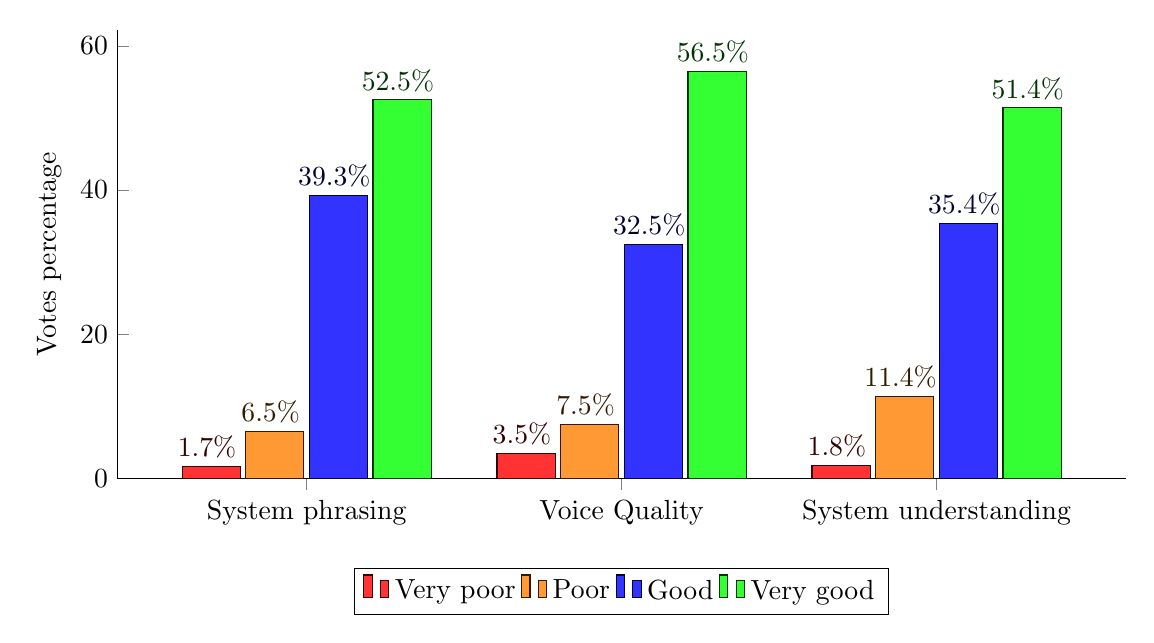
\begin{tikzpicture}
\begin{axis}[
    every axis plot post/.style={/pgf/number format/fixed},
    ybar,
    x=4cm,
    ymin=0,
    ylabel = Votes percentage,
    %ymax=12,
    legend columns=-1,
	legend style={at={(0.5,-0.2)},anchor=north},
    xtick=data,
    enlarge x limits=0.3,
    bar width=21pt,
    symbolic x coords={1, 2, 3, 4},
    nodes near coords={\pgfmathprintnumber\pgfplotspointmeta\%},
    nodes near coords align={
     shift={(-0.15em,0.7em)},
    },
    axis lines*=left,
    xticklabels={System phrasing, Voice Quality, System understanding},
    xtick={1,...,3},
    ]
\addplot[red!20!black,fill=red!80!white] coordinates {(1,1.7) (2,3.5) (3,1.8)};
\addplot[orange!20!black,fill=orange!80!white] coordinates {(1,6.5) (2,7.5) (3,11.4)};
\addplot[blue!20!black,fill=blue!80!white] coordinates {(1,39.3) (2,32.5) (3,35.4)};
\addplot[green!20!black,fill=green!80!white] coordinates {(1,52.5) (2,56.5) (3,51.4)};
\legend{Very poor, Poor, Good, Very good}
\end{axis}
\end{tikzpicture}
\caption{Kaldi subjective user satisfaction histograms for questions 2-4 from table \ref{table:cf}}
\label{fig:kaldi}
\end{figure}


The figure \ref{fig:kaldi} shows histograms for questions 2, 3 and 4.
It is clear that very few contributors were unsatisfied with the service.
It indicates an improvement in comparison to the Google \ac{ASR}.
The first yes-no overall question is shown in figure \ref{fig:us}.

Only 60 contributors decided to write a general comment which were generally positive.

\begin{flushleft}
\textit{``Good, fast service.''} \\
\textit{``I liked this.''} \\
\textit{``It would be nice if the voice was more fluid. It sounds too robotic.''} \\
\textit{``Wow! An automated system that understands my needs!''} \\
\end{flushleft}

\noindent This also indicates an improvement against the Google \ac{ASR}.

\section{Comparison -- summary}

It is clear that the system was able to respond both with Google and Kaldi \ac{ASR}.
Although notably better results were achieved with Kaldi \ac{ASR} as the subjective user satisfaction displayed in figure \ref{fig:us} is in favor of Kaldi \ac{ASR}.

\begin{figure}[ht]
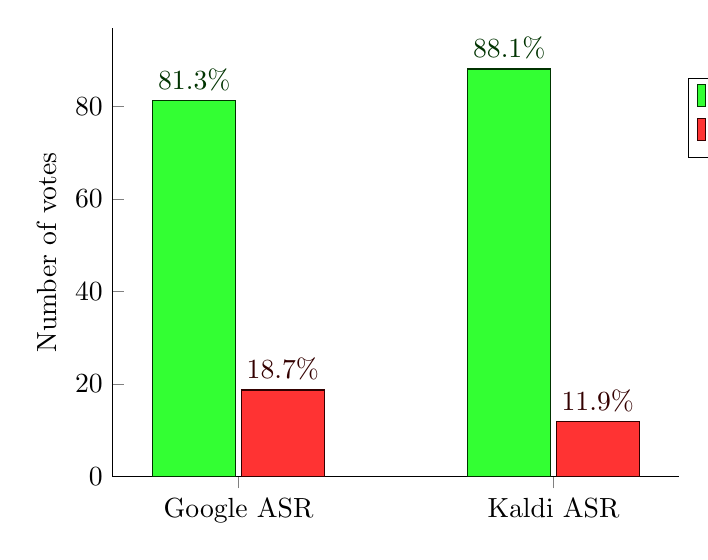
\begin{tikzpicture}
\begin{axis}[
    every axis plot post/.style={/pgf/number format/fixed},
    ybar,
    x=4cm,
    ymin=0,
    ylabel = Number of votes,
    %xlabel = Found what was looking for,
    %ymax=12,
    legend columns=1,
	legend style={
         overlay,
         at={(1.1,0.8)},
         anchor=center},
    xtick=data,
    enlarge x limits=0.4,
    bar width=30pt,
    symbolic x coords={1, 2},
    nodes near coords={\pgfmathprintnumber\pgfplotspointmeta\%},
    axis lines*=left,
    xticklabels={Google ASR, Kaldi ASR},
    xtick={1,...,2},
    ]

\addplot[green!20!black,fill=green!80!white] coordinates {(1,81.3) (2,88.1)};
\addplot[red!20!black,fill=red!80!white] coordinates {(1,18.7) (2,11.9)};
\legend{Yes, No}
\end{axis}
\end{tikzpicture}
\caption{User satisfaction, have found what they were looking for}
\label{fig:us}
\end{figure}

Callers communicating with \ac{PTINY} using Google \ac{ASR} did obtain what they were looking for in $81.3\%$.
Whereas Kaldi \ac{ASR} callers were satisfied in $88.1\%$.
Means and standard deviances of individual questions are displayed in table \ref{table:mv}.
The mean of all the questions increased with Kaldi \ac{ASR} while the standard deviance of each question decreased.

\begin{table}[h]
\centering
\begin{tabular}{l|ll|ll}
                     & \multicolumn{2}{c |}{\textbf{Google}}  & \multicolumn{2}{c}{\textbf{Kaldi}}   \\ \hline
                     & \textbf{Mean}         & \textbf{StD}          & \textbf{Mean}         & \textbf{StD}          \\ \hline
\textit{System phrasing}      & 3.17 & 0.91 & 3.43 & 0.69 \\
\textit{Voice Quality}        & 3.07 & 0.95 & 3.42 & 0.78 \\
\textit{System understanding} & 3.03 & 0.98 & 3.36 & 0.76 \\
\textit{Overall performance}  & 0.81 & 0.39 & 0.88 & 0.32
\end{tabular}
\caption[Mean and standard deviation of Google and Kaldi ASR]{Mean and standard deviation comparison of Google and Kaldi ASR}
\label{table:mv}
\end{table}

The measurement for the question number 2, evaluating the voice quality, were following the improving tendency of the other questions.
The \ac{TTS} component, however, was still the same.
This phenomenon could be caused by the user satisfaction from completing the job with ease.
When \ac{ASR} does not recognize an utterance the \ac{DM} does not change the state and the user needs to repeat himself.
This can be annoying and ultimately, it may be reflected on the feedback.

\subsubsection{\ac{ASDF} \ac{ASR} comparison}

We compared both \ac{ASR} components individually, isolated them from the dialogue system.
\ac{ASDF} allows us to divide the transcriptions from call logs into training and testing sets along with respective audio tracks.
After training \ac{LM} and building Kaldi decoder, we were able to test it on unseen utterances and compare it with Google \ac{ASR}.

The measure we were concerned with was \acf{WER}.
\ac{WER} of Google \ac{ASR} was $31.33\%$ while \ac{WER} of Kaldi \ac{ASR} was $16.93\%$.
This indicates that adapted Kaldi \ac{ASR} was much better on all of 149 test utterances.

\section{Future work}

The provided \ac{PTINY} solution would benefit from further \ac{SLU}, \ac{NLG}  and static knowledge database improvements for covering another area.
Utilizing \ac{MTA} \ac{API} would furnish real-time information about connections, for example current position of train.
The route descriptions can be really extensive, therefore it would be a valuable feature to send the directions in SMS form on demand.
Statistical \ac{SLU} for robustness may be also profitable to develop.
